\section{Bitcoin}
Bitcoin was introduced in 2008 by Satoshi Nakamoto~\cite{bitcoin} as a
peer-to-peer version of electronic cash, allowing online payments to be sent
directly between parties without the need of a intermediary.

Transfer of value in Bitcoin happens with transactions. A transaction has
inputs and outputs. An output is where the value creation happens for the
receiver. An output can be later redeemed by using its designated receiver's
private key and turned into an input to be used for another transaction.

TODO

\subsection{Block Structure}
A block header contains mainly the hash of the previous block, a Merkle root
hash to commit to a set of transactions, and a nonce.

After the block header comes the series of transactions included in the block.

TODO

\subsection{Proof of Work}
\subsection{Merkle Trees}
A Merkle tree~\cite{merkle} is a data structure which allows a party to
commit to a set of items using only a single hash, and prove the inclusion of
any item in the committed set by providing a logarithmic proof in terms of the
cardinality of the set.

More specifically, the hashes of the items consist the leafs of the tree, and
the last level. The internal levels are defined recursively as follows: To
create level $k-1$ each pair of level $k$ $(A, B)$ is transformed as a node
of value $H(A || B)$ which points to both $A$ and $B$. If the number of nodes
at level $k$ is odd, the last node at that level is paired with itself.
\footnote{This specific construction is the one Bitcoin implements. There are
various other constructions which are not inside the scope of this paper.}

Merkle trees are useful in Bitcoin in order to commit to a set of
transactions to be included in a block while keeping the block header of a
constant size.

To provide proof of inclusion, all a prover has to do is provide a path of
siblings up to the root $\sf{siblings}$ and a bit vector $\sf{left}$ indicating
whether each sibling is on the left or the right. The verification process is
shown in Algorithm~\ref{alg:merkle-verification}.

\begin{algorithm}[H]
  \caption{\label{alg:merkle-verification}The \textsf{Verify} algorithm
    for a Merkle proof}
    \begin{algorithmic}[1]
      \Function{\sf Verify$_{\sf root}$}{\sf leaf, siblings, left}
            \Let{\sf{currentHash}}{\sf{leaf}}
            \While{$\sf{left} \neq []$}
              \Let{\sf{siblingIsLeft}}{\sf{left.shift()}}
              \If{\sf{siblingIsLeft}}
                \Let{\sf{currentHash}}{H(siblings.shift() || currentHash)}
              \Else
                \Let{\sf{currentHash}}{H(currentHash || siblings.shift())}
              \EndIf
            \EndWhile
            \State\Return{currentHash = root}
        \EndFunction
    \end{algorithmic}
\end{algorithm}

An example of a Bitcoin Merkle tree, along with a proof of inclusion for $K$ can be seen on Figure~\ref{fig:merkletree}.

\begin{figure}
  \centering
  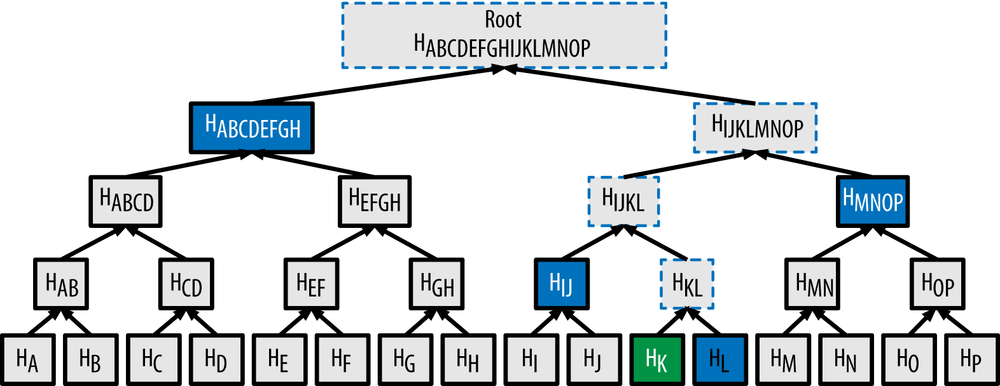
\includegraphics[width=0.9\columnwidth,keepaspectratio]{figures/merkle-tree-proof.png}
  \caption{A Bitcoin Merkle tree. Source:~\cite{mastering}}
  \label{fig:merkletree}
\end{figure}

\subsection{Simplified Payment Verification}
The size of the blockchain has reached 185GB by September 2018, which makes
it a very time consuming or even infeasible process to synchronise a full
node. Fortunately, a solution was proposed in the original whitepaper
~\cite{bitcoin}, which allows the creation of so-called \textit{lite nodes}.
Lite nodes only know the headers of the entire blockchain, which are
constant-size for each block (80 bytes). At the time of writing of this
paper, the size of all block headers was $\sim$42MB. The lite node then asks the
network for transactions concerning it (e.g.\ transactions concerning a
specific public key). Full nodes of the network find such transactions and
return them to the requester. For each transaction, the block header of the
block it's included in is returned, along with a Merkle tree proof of
inclusion which the lite node can then verify. This protocol is reliable as
long as an adversary does not control the network of a lite node.

\subsection{Bitcoin Cash}
In 2017 Bitcoin faced severe scalability issues~\cite{onscaling}. Its limited
1MB block size meant that it could only support a maximum of 7 transactions per
second. As Bitcoin's popularity had exploded at the time, the problem was
hugely exacerbated. The most prominently proposed solution for this was a block
size increase, however no consensus was reached. The discussions ended with a
fork of the main Bitcoin chain which allowed for 8MB blocks, called Bitcoin
Cash.
